\documentclass[tikz,border=4pt]{standalone}
% Estilos compartilhados pelos diagramas dos estágios e módulos do Core.
\usetikzlibrary{arrows.meta, positioning, calc, shapes.geometric, fit}

\tikzset{
  >={Stealth[length=2.2mm]},
  bloco/.style={draw, rounded corners=2pt, minimum width=24mm, minimum height=9mm,
                align=center, font=\small, fill=blue!6},
  regpipe/.style={draw, minimum width=9mm, minimum height=48mm, align=center,
                  font=\small, fill=gray!25},
  mux/.style={draw, trapezium, trapezium angle=70, shape border rotate=90,
              minimum height=11mm, minimum width=7mm, inner sep=1pt, align=center,
              font=\scriptsize, fill=orange!15},
  ctrl/.style={draw, rounded corners=2pt, minimum width=24mm, minimum height=9mm,
               align=center, font=\small, fill=green!10},
  opcional/.style={bloco, dashed, fill=yellow!12},
  externo/.style={draw, rounded corners=2pt, minimum width=24mm, minimum height=9mm,
                  align=center, font=\small, fill=red!8},
  dado/.style={->, thick},
  sinal/.style={->, dashed},
  rotulo/.style={font=\scriptsize, midway, above, inner sep=1pt},
  titulo/.style={font=\bfseries\normalsize}
}

\begin{document}
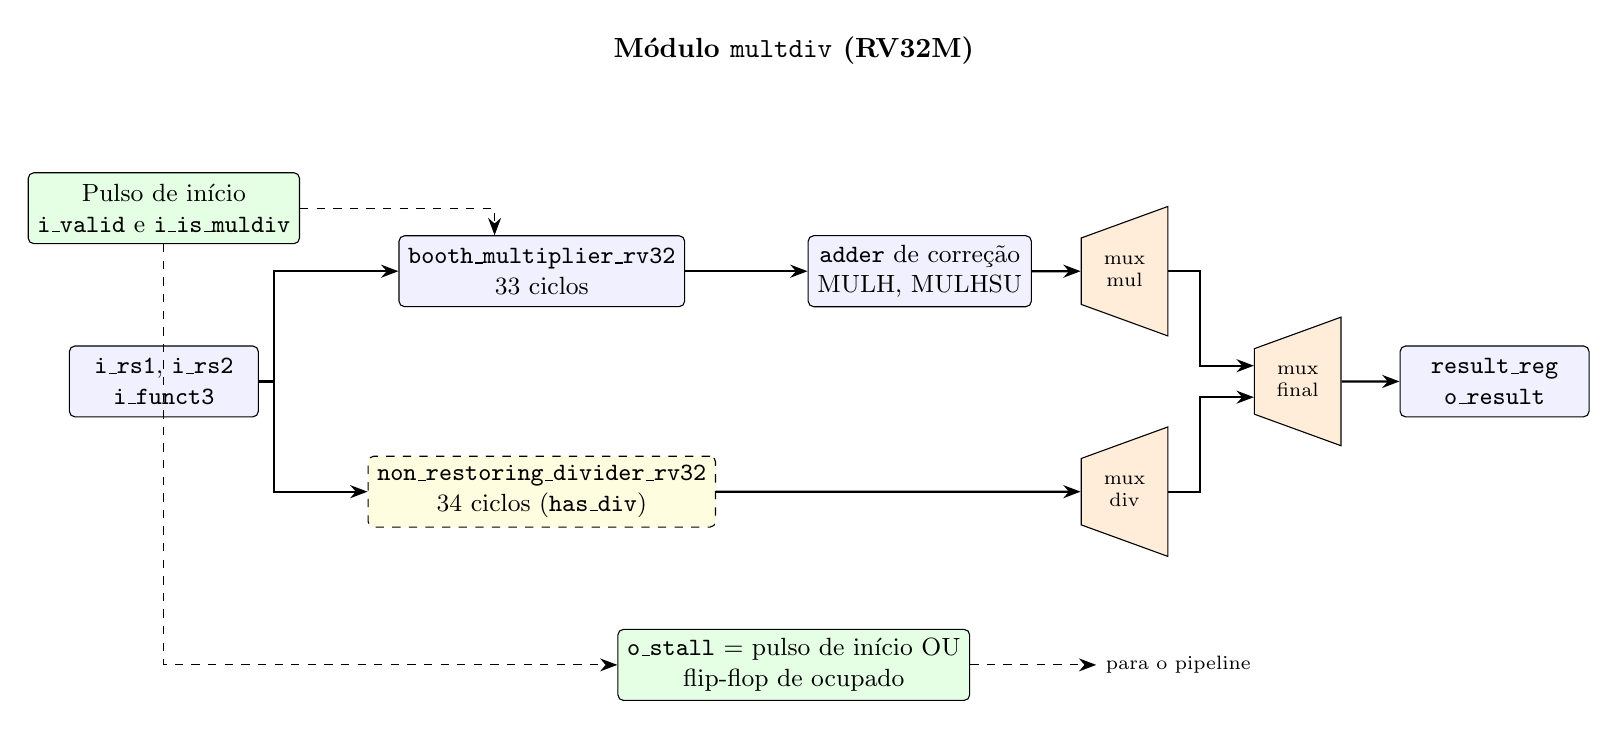
\begin{tikzpicture}
  \node[titulo] at (8,6.4) {Módulo \texttt{multdiv} (RV32M)};
  \node[bloco] (in) at (0,2.2) {\texttt{i\_rs1}, \texttt{i\_rs2}\\\texttt{i\_funct3}};
  \node[ctrl] (start) at (0,4.4) {Pulso de início\\\texttt{i\_valid} e \texttt{i\_is\_muldiv}};
  \node[bloco] (booth) at (4.8,3.6) {\texttt{booth\_multiplier\_rv32}\\33 ciclos};
  \node[opcional] (div) at (4.8,0.8) {\texttt{non\_restoring\_divider\_rv32}\\34 ciclos (\texttt{has\_div})};
  \node[bloco] (corr) at (9.6,3.6) {\texttt{adder} de correção\\MULH, MULHSU};
  \node[mux] (mm) at (12.2,3.6) {mux\\mul};
  \node[mux] (dm) at (12.2,0.8) {mux\\div};
  \node[mux] (fm) at (14.4,2.2) {mux\\final};
  \node[bloco] (res) at (16.9,2.2) {\texttt{result\_reg}\\\texttt{o\_result}};
  \node[ctrl] (stall) at (8,-1.4) {\texttt{o\_stall} = pulso de início OU\\flip-flop de ocupado};

  \draw[dado] (in) -- ++(1.4,0) |- (booth.west);
  \draw[dado] (in) -- ++(1.4,0) |- (div.west);
  \draw[sinal] (start) -- (booth.north west |- start.east) -| ([xshift=-6mm]booth.north);
  \draw[dado] (booth.east) -- (corr.west);
  \draw[dado] (corr.east) -- (mm.west);
  \draw[dado] (div.east) -- (dm.west);
  \draw[dado] (mm.east) -- ++(0.4,0) |- ([yshift=2mm]fm.west);
  \draw[dado] (dm.east) -- ++(0.4,0) |- ([yshift=-2mm]fm.west);
  \draw[dado] (fm) -- (res);
  \draw[sinal] (start.south) |- (stall.west);
  \draw[sinal] (stall.east) -- ++(1.6,0) node[font=\scriptsize, right] {para o pipeline};
\end{tikzpicture}
\end{document}
